\usetikzlibrary{patterns} % la librairie qui permet de remplir avec des motifs, cf le manuel : https://tex.stackexchange.com/questions/29808/can-i-control-the-density-of-a-pattern-in-tikz

% Pour personnaliser éventuellement les hachures : https://tex.stackexchange.com/questions/29808/can-i-control-the-density-of-a-pattern-in-tikz


% Autre fonction utile : la fonction clip, qui permet de découper une partie de dessin selon une géométrie
%
%
%INCLUDE ONCE

\tikzset{
    hatch distance/.store in=\hatchdistance,
    hatch distance=10pt,
    hatch thickness/.store in=\hatchthickness,
    hatch thickness=0.3pt
}

\makeatletter
\pgfdeclarepatternformonly[\hatchdistance,\hatchthickness]{northeast}
{\pgfqpoint{0pt}{0pt}}
{\pgfqpoint{\hatchdistance}{\hatchdistance}}
{\pgfpoint{\hatchdistance-1pt}{\hatchdistance-1pt}}%
{
    \pgfsetcolor{\tikz@pattern@color}
    \pgfsetlinewidth{\hatchthickness}
    \pgfpathmoveto{\pgfqpoint{0pt}{0pt}}
    \pgfpathlineto{\pgfqpoint{\hatchdistance}{\hatchdistance}}
    \pgfusepath{stroke}
}

\pgfdeclarepatternformonly[\hatchdistance,\hatchthickness]{northwest}
{\pgfqpoint{0pt}{0pt}}
{\pgfqpoint{\hatchdistance}{\hatchdistance}}
{\pgfpoint{\hatchdistance-1pt}{\hatchdistance-1pt}}%
{
    \pgfsetcolor{\tikz@pattern@color}
    \pgfsetlinewidth{\hatchthickness}
    \pgfpathmoveto{\pgfqpoint{\hatchdistance}{0pt}}
    \pgfpathlineto{\pgfqpoint{0pt}{\hatchdistance}}
    \pgfusepath{stroke}
}

\pgfdeclarepatternformonly[\hatchdistance,\hatchthickness]{horizontal}
{\pgfqpoint{0pt}{0pt}}
{\pgfqpoint{\hatchdistance}{\hatchdistance}}
{\pgfpoint{\hatchdistance-1pt}{\hatchdistance-1pt}}%
{
    \pgfsetcolor{\tikz@pattern@color}
    \pgfsetlinewidth{\hatchthickness}
    \pgfpathmoveto{\pgfqpoint{0pt}{0pt}}
    \pgfpathlineto{\pgfqpoint{\hatchdistance}{0pt}}
    \pgfusepath{stroke}
}

\pgfdeclarepatternformonly[\hatchdistance,\hatchthickness]{vertical}
{\pgfqpoint{0pt}{0pt}}
{\pgfqpoint{\hatchdistance}{\hatchdistance}}
{\pgfpoint{\hatchdistance-1pt}{\hatchdistance-1pt}}%
{
    \pgfsetcolor{\tikz@pattern@color}
    \pgfsetlinewidth{\hatchthickness}
    \pgfpathmoveto{\pgfqpoint{0pt}{0pt}}
    \pgfpathlineto{\pgfqpoint{0pt}{\hatchdistance}}
    \pgfusepath{stroke}
}
\makeatother


\begin{center}
\resizebox{\linewidth}{!}{
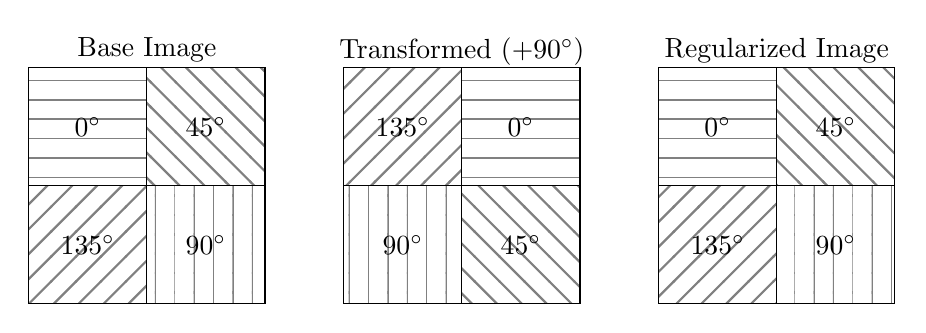
\begin{tikzpicture}

\draw[pattern=horizontal,pattern color=gray,hatch distance=8pt, hatch thickness = 0.8pt]  (0,1.5) rectangle (1.5,3)node[midway]{$0^\circ$}; % texte avec fond
 \draw[pattern=northwest,pattern color=gray,hatch distance=10pt, hatch thickness = 0.8pt] (1.5,1.5) rectangle (3,3) node[midway]{$45^\circ$};
 \draw[pattern=vertical,pattern color=gray,hatch distance=8pt, hatch thickness = 0.8pt](1.5,0) rectangle (3,1.5)
node[midway]{$90^\circ$};
\draw[pattern=northeast,pattern color=gray,hatch distance=10pt, hatch thickness = 0.8pt]  (0,0) rectangle (1.5,1.5)
node[midway]{$135^\circ$};

\draw (1.5,3.5) node[below]{Base Image};

\begin{scope}[shift={(4,0)}]

\draw[pattern=horizontal,pattern color=gray,hatch distance=8pt, hatch thickness = 0.8pt]  (1.5,1.5) rectangle (3,3)node[midway]{$0^\circ$}; % texte avec fond
 \draw[pattern=northwest,pattern color=gray,hatch distance=10pt, hatch thickness = 0.8pt] (1.5,0) rectangle (3,1.5) node[midway]{$45^\circ$};
 \draw[pattern=vertical,pattern color=gray,hatch distance=8pt, hatch thickness = 0.8pt](0,0) rectangle (1.5,1.5)
node[midway]{$90^\circ$};
\draw[pattern=northeast,pattern color=gray,hatch distance=10pt, hatch thickness = 0.8pt]  (0,1.5) rectangle (1.5,3)
node[midway]{$135^\circ$};

\draw (1.5,3.5) node[below]{Transformed ($+90^\circ$)};

\end{scope}

\begin{scope}[shift={(8,0)}]

\draw[pattern=horizontal,pattern color=gray,hatch distance=8pt, hatch thickness = 0.8pt]  (0,1.5) rectangle (1.5,3)node[midway]{$0^\circ$}; % texte avec fond
 \draw[pattern=northwest,pattern color=gray,hatch distance=10pt, hatch thickness = 0.8pt] (1.5,1.5) rectangle (3,3) node[midway]{$45^\circ$};
 \draw[pattern=vertical,pattern color=gray,hatch distance=8pt, hatch thickness = 0.8pt](1.5,0) rectangle (3,1.5)
node[midway]{$90^\circ$};
\draw[pattern=northeast,pattern color=gray,hatch distance=10pt, hatch thickness = 0.8pt]  (0,0) rectangle (1.5,1.5)
node[midway]{$135^\circ$};

\draw (1.5,3.5) node[below]{Regularized Image};

\end{scope}

\end{tikzpicture}
}
\end{center}

